\section{Study Workflow}

Figure~\ref{fig:workflow} summarizes our three-stage workflow. First, \emph{Repository Bug Collection} identifies and verifies merged bug-fixing PRs. Second, \emph{Bug Evidence Integration \& Validation} assigns the required manual labels and links them with repository evidence and patch information to construct one validated record for each verified fix. Third, \emph{Empirical Analysis} uses these records to study failure localization, repair structure, and repair evolution. The unit of analysis throughout the study is a merged PR that was manually verified to repair a bug.

\begin{figure*}[t]
    \centering
    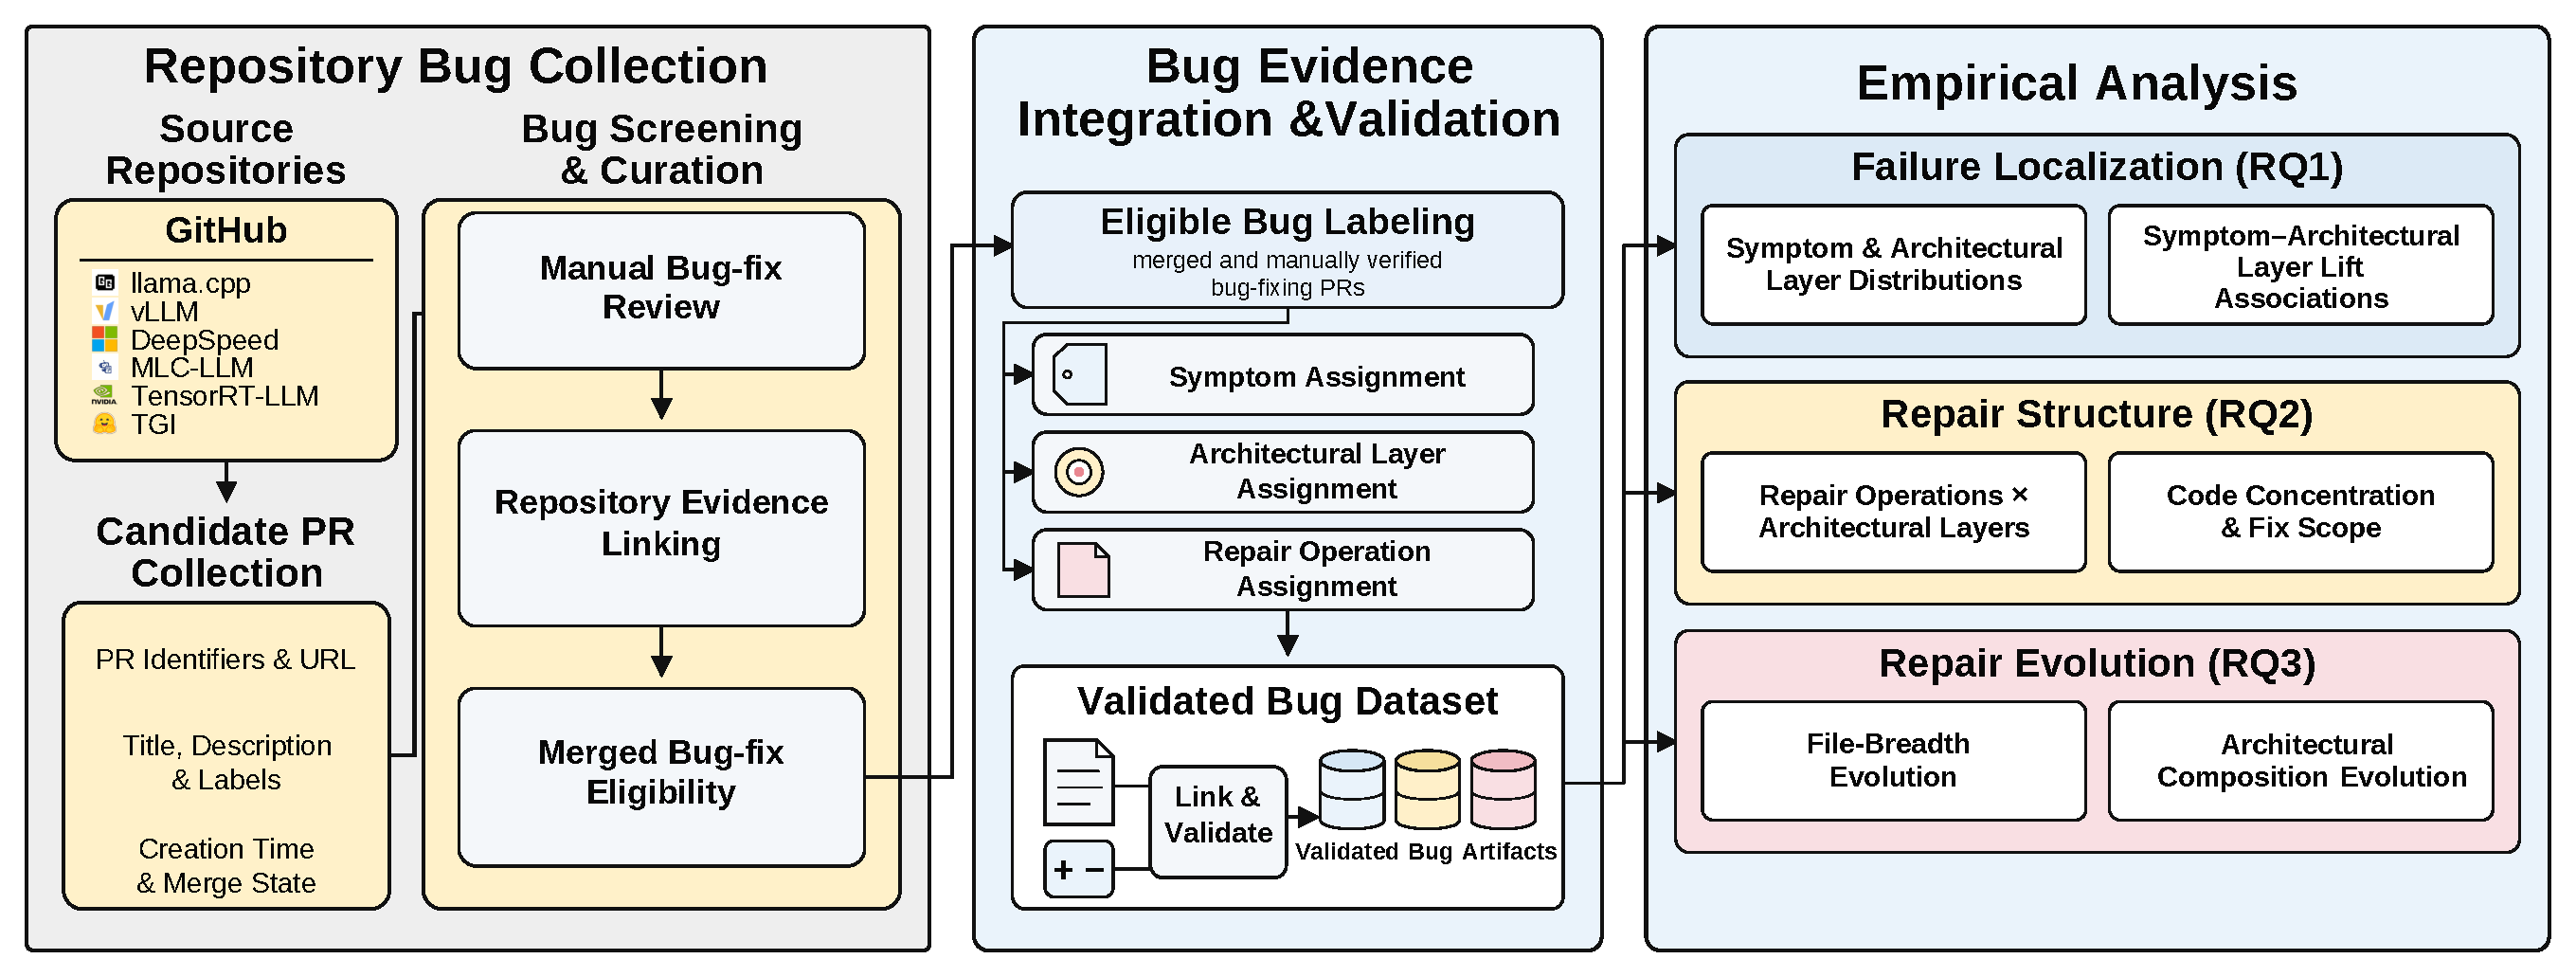
\includegraphics[width=\textwidth]{fig/workflow.pdf}
    \caption{Three-stage workflow of the empirical study: repository bug collection, bug-evidence integration and validation, and empirical analysis.}
    \label{fig:workflow}
\end{figure*}

\subsection{Repository Bug Collection}

\textbf{Source Repositories.} We study six widely used open-source engines for LLM inference: llama.cpp, vLLM, DeepSpeed, MLC-LLM, TensorRT-LLM, and Text Generation Inference (TGI). They represent the engine landscape surveyed in prior work~\cite{park2026inferenceengines} and cover local inference, high-throughput serving, compiler-based deployment, distributed execution, and hardware-specific acceleration. We use each project's official GitHub repository and include PRs from its earliest available records through March 2026. Table~\ref{tab:bug_stats} reports the period covered for each repository.

We collected 50,121 candidate bug-fixing PRs from the six repositories. For each PR, we recorded its repository and PR identifiers, URL, title, description, labels, and creation time. We did not rely solely on GitHub's bug labels because they are incomplete and may misclassify changes~\cite{bird2009mininggit,herzig2013misclassification}.


\begin{table}[t]
  \centering
  \caption{Study corpus by project.}
  \label{tab:bug_stats}
  \begin{tabular}{l c r r}
    \toprule
    Engine & Time frame & \# Candidates & \# Fixes \\
    \midrule
    llama.cpp    & Mar. 2023--Mar. 2026 & 10,549 & 3,004 \\
    vLLM         & Feb. 2023--Mar. 2026 & 23,561 & 5,915 \\
    DeepSpeed    & Jan. 2020--Mar. 2026 &  3,683 & 1,118 \\
    MLC-LLM      & Apr. 2023--Mar. 2026 &  1,816 &   487 \\
    TensorRT-LLM & Aug. 2023--Mar. 2026 &  8,802 & 1,784 \\
    TGI          & Oct. 2020--Mar. 2026 &  1,710 &   399 \\
    \midrule
    \textbf{Total} & --- & \textbf{50,121} & \textbf{12,707} \\
    \bottomrule
  \end{tabular}
\end{table}

\textbf{Bug Screening \& Curation.} Two experts with LLM inference-engine development experience independently reviewed each candidate PR. They examined the PR title and description, development discussion, linked issue, and complete patch to determine whether the change repaired an actual software defect. A PR was considered bug-fixing only when its evidence and patch established that it corrected unintended behavior; feature additions and other changes without evidence of defect correction were rejected. The experts discussed every disagreement until reaching consensus.

We linked each collected PR record to its development discussion, linked issue when available, complete patch, and GitHub merge state. We then combined these artifacts with the consensus screening decision, producing a traceable evidence record for each candidate rather than treating a repository label or PR description as sufficient evidence on its own.

The final corpus retains a PR only when it was both confirmed as bug-fixing through the review above and merged into the corresponding project codebase. This procedure produced 12,707 merged and manually verified bug-fixing PRs, distributed across the six projects as shown in Table~\ref{tab:bug_stats}.
\subsection{Bug Evidence Integration \& Validation}

\textbf{Eligible Bug Labeling.} The labels needed by our RQs cannot be recovered reliably from repository metadata alone. Symptoms describe externally observed failures, whereas architectural layers and repair operations require interpreting the development discussion together with the patch. We therefore derived the coding scheme directly from the collected PR evidence instead of treating GitHub labels as ground truth.

The two experts first reviewed an initial set of 1,000 PRs and used iterative open coding, following established guidance for qualitative empirical software-engineering research~\cite{seaman1999qualitative}, to derive candidate categories. They compared the proposed categories, discussed their boundaries, and repeatedly merged, split, or refined them when a category was ambiguous or failed to distinguish technically different cases. This process continued until the coding scheme stabilized, yielding ten symptom categories, nine architectural-layer categories, and nine repair-operation categories. The resulting taxonomies are grounded in recurring evidence from real fixes while retaining a common vocabulary applicable across all engines.

We assign one \emph{symptom} to each bug, representing the primary failure visible to a user or developer before the repair. We assign one \emph{repair operation}, representing the principal corrective action performed by the patch. Architectural-layer assignment is multi-label because a defect may span several architectural regions; accordingly, each bug is assigned one or more \emph{architectural layers} containing the faulty logic or state responsible for the failure. Architectural-layer labels identify faulty locations rather than indiscriminately treating every file modified by a patch as a fault location.

After the taxonomies were finalized, the two experts independently applied them to the complete corpus. Each decision was based on the same evidence used for eligibility review: the PR description, discussion, linked issue, and complete patch. They then compared their labels and resolved disagreements through discussion until consensus.

\textbf{Evidence Integration.} For each verified fix, this stage combines repository metadata, development discussion, linked issues when available, the complete patch, and the consensus labels produced through the labeling procedure above. We link these artifacts by repository and PR identifier and consolidate them into one structured record per fix. Each record preserves the PR URL and creation time, the evidence used during review, one symptom, one repair operation, one or more architectural layers, and the patch metadata required to measure modified entities and fix scope.

\textbf{Record Validation.} We validate each integrated record against the eligibility decision established during screening and the consensus labels produced through the labeling procedure above. In particular, the record must refer to a merged PR, carry the consensus bug-fixing decision and required labels, and link to the patch reviewed by the experts. The resulting analysis-ready dataset contains 12,707 validated records. Architectural layers are retained as a list within a single bug record rather than expanded into duplicate rows; the weighting or expansion required by a particular analysis is applied explicitly in the next stage. This preserves a stable denominator while allowing RQ1 and RQ2 to use different multi-layer counting rules.
%The collection stage produces several artifacts for each verified fix: repository metadata, development discussion, linked issues when available, the complete patch, and consensus labels. We link these artifacts by repository and PR identifier and consolidate them into one structured record per fix. Each record preserves the PR URL and creation time, the evidence used during review, one symptom, one repair operation, one or more architectural layers, and the patch metadata required to measure modified entities and fix scope.

%We validate the integrated record against the evidence and eligibility decisions established in the previous stage. In particular, the record must refer to a merged PR, carry the consensus bug-fixing decision and required labels, and link to the patch reviewed by the experts. The resulting dataset contains 12,707 validated records. Root-cause layers are retained as a list within a single bug record rather than expanded into duplicate rows; the weighting or expansion required by a particular analysis is applied explicitly in the next stage. This preserves a stable denominator while allowing RQ1 and RQ2 to use different multi-layer counting rules.


\subsection{Empirical Analysis}

The final stage answers the three research questions through complementary analyses. RQ1 relates externally observed symptoms to the architectural layers containing the faulty code. RQ2 characterizes how repairs are structured across repair operations, architectural layers, and code entities. RQ3 tracks how repair scope evolves over time.

\textbf{Failure Localization (RQ1).} To characterize where failures manifest and where their underlying faults reside, we compute the distributions of symptoms and architectural layers for each project and for the combined corpus. Because a bug may have multiple architectural layers, counting it once in every assigned layer would give multi-layer bugs disproportionate influence. We therefore assign a weight of $1/k$ to each of a bug's $k$ architectural layers, keeping the bug's total weight at one.

We quantify the association between a symptom $s$ and an architectural layer $l$ using lift. Let $w_{s,l}$ be the weighted number of bugs having symptom $s$ and layer $l$, $w_s$ the total weight of bugs with symptom $s$, $w_l$ the total weight assigned to layer $l$, and $W$ the total weight of all verified bugs. We compute
\begin{equation}
    \operatorname{Lift}(s,l)
    = \frac{P(l\mid s)}{P(l)}
    = \frac{w_{s,l}/w_s}{w_l/W}.
\end{equation}
A lift greater than one indicates that layer $l$ is overrepresented among bugs with symptom $s$ relative to its prevalence in the full corpus; a value below one indicates underrepresentation. We use lift as a descriptive association measure and do not interpret it as evidence of causality.

\textbf{Repair Structure (RQ2).} We characterize how bug-fixing work is structured across architectural layers and code entities from three complementary perspectives. First, we cross-tabulate repair operations with architectural layers. Although each bug has exactly one repair operation, a bug assigned to $k$ architectural layers contributes one repair-operation instance to each of those layers. Consequently, the 12,707 fixes yield 19,965 repair-operation instances. This rule includes every affected layer in the repair-operation counts.

Second, we measure code concentration at file and function granularity. Prior work has shown that fault-prone locations and change history are useful signals for focusing quality-assurance effort~\cite{ostrand2005faultlocation,graves2000changehistory}. For each project, we count the bug-fixing occurrences associated with each entity, rank entities in descending order, and construct cumulative concentration curves. We report the fraction of all bug-fixing occurrences covered by the top 20\% of files and functions, as well as the fraction of entities required to cover 80\% of the occurrences.

Third, we quantify the scope of each fix using changed lines and modified files. Changed lines are the sum of added and deleted lines in the complete PR patch, whereas the number of modified files captures how broadly the repair spreads across the repository. These change-level measures are consistent with prior just-in-time quality-assurance research that treats properties of individual changes as review and testing signals~\cite{kamei2013jitqa}. They describe repair scope rather than bug severity. Because fix sizes are strongly right-skewed, we characterize their distribution using the median and upper quantiles instead of relying on the mean. For RQ3, we pair these patch-level measures with layer-level fix distributions.

Because their units differ, we keep the three RQ2 measures separate. Repair-operation instances count actions in each affected layer; entity concentration records repeated changes to files and functions; changed lines and modified files describe a complete fix. A combined score would blur important distinctions: a large patch is not necessarily severe, a frequently modified entity is not faulty in every PR, and a multi-layer fix is not several independent bugs.

\textbf{Repair Evolution (RQ3).} To examine how repair scope evolves over time, we group fixes by the month when their PR was created. Several projects have few monthly observations before 2023, so the trend analysis covers January 2023 through March 2026. For each month, we group fixes by the number of modified files---one file, two to five files, or at least six files---and track the share of each group. We also track the share of bug-fixing activity in each architectural layer. We first remove duplicate layer labels for each bug. We then split its weight equally among those layers, keeping the total at one.

To test whether each monthly layer share generally increases or decreases over time, we compute Spearman's rank correlation between the month number and the layer share. Let $t\in\{1,\ldots,n\}$ be the month number, where $n=39$, and let $Y_t$ be the weighted share of a layer in month $t$. If $R_t$ is the rank of month $t$ and $S_t$ is the rank of $Y_t$, with average ranks for tied values, the correlation is
\begin{equation}
\rho =
\frac{\sum_{t=1}^{n}(R_t-\bar{R})(S_t-\bar{S})}
{\sqrt{\sum_{t=1}^{n}(R_t-\bar{R})^2}
 \sqrt{\sum_{t=1}^{n}(S_t-\bar{S})^2}}.
\label{eq:spearman_temporal}
\end{equation}
A positive $\rho$ indicates that the layer's monthly share tends to increase over time, whereas a negative value indicates that it tends to decrease. We use Spearman's correlation because it can capture a general upward or downward trend without assuming a straight-line relationship or a normal distribution of monthly values. For each layer, we obtain a two-sided $p$-value for the null hypothesis $H_0:\rho=0$ using 20,000 random permutations. Because we test nine architectural layers, some trends may appear significant by chance. We therefore apply the Benjamini--Hochberg procedure~\cite{benjamini1995controlling} to the nine $p$-values, control the false discovery rate---the expected share of false positives among trends declared significant---at 0.05, and report the adjusted values as $q$-values. We also report the least-squares slope in percentage points per year to make the size of each change easier to understand.

To check whether an overall trend is caused by changes in the mix of projects, we recompute the monthly layer shares for each project and combine them using fixed project weights based on the full analysis period. When a project has no fixes in a month, we adjust the weights of the active projects so that they still sum to one. Because we use the PR creation date, this analysis shows how observed bug-fixing activity changes over time. It does not measure when bugs were introduced, how long they took to discover, or how long they took to repair.
